
%mainfile: Spikes.tex

\pagestyle{fancy} 
\lhead{Atelier Nueromodélisation, 2017}
\rhead{Problem set \#3}
\rfoot{\thepage}
\cfoot{}
\lfoot{}
\renewcommand{\headrulewidth}{0.4pt}
\renewcommand{\footrulewidth}{0.4pt}


\title{Problem Set \#3: Spikes \vspace{-0.5em}}
\preauthor{} \postauthor{} 
\author{}
\date{\today}
\maketitle

\thispagestyle{fancy}


\section*{Introduction}

Neurons in our brain need to fire signals to communicate with each other. 
These signals, electrochemical in nature, are refered to as spikes, or action
potentials. Here we'll look at several different aspects of this essential
element in our nervous system.


\section{Spike trains}

\subsection{Poisson Model}

Before discussing how spikes are produced, we'll first work on the
statistical description of spike trains (i.e. a seqeunce of spikes and 
silences from a single neuron). As a first approximation, the generation of 
a random spike train can be simulated by a Poisson process. We assume that
individual spikes are generated mutaually independently with some probability 
that can be deduced from the instantaneous firing rate. 

Since the computer is a discret system, a spike train will just be modeled as
an array of 0s and 1s. For example, we create a vector of 1000 elements 
such that each element of the vector has 25\% to be 1.

\begin{figure}[H]
  \centering
  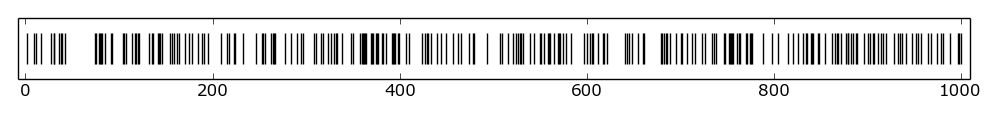
\includegraphics[width=0.9\linewidth]{stPoisson1}
  \caption{A Bernoulli process of 1000 trials with $p = 0.25$}
\end{figure}

Next we introduce time units, every 0 or 1 is assocaited with a time bin 
of lenght $\Delta t$ ms. Here we choose $\Delta t = 2$ ms and generate a spike
train of length 1 sec with the firing rate 25 spikes/sec.

\begin{figure}[H]
  \centering
  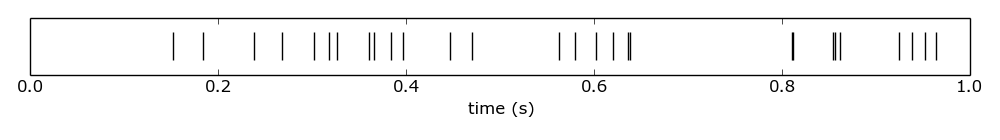
\includegraphics[width=0.9\linewidth]{stPoisson2}
  \caption{A Poisson spike train with an average rate of 25 spikes/sec}
\end{figure}

In the above figure, there are in effect 28 spikes that are generated. We may
be insterested in the distribution of the total number of spikes in each
simulation that we refer to as total spike count here. Thus we'll generate 50
spike trains with the same parameters.

\begin{figure}[H]
  \centering
  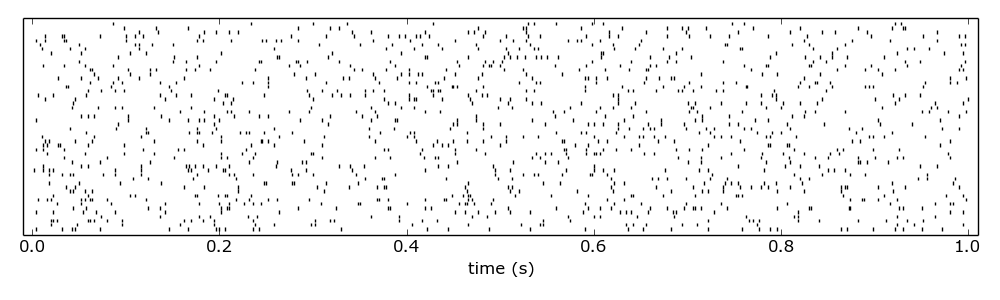
\includegraphics[width=0.9\linewidth]{stPoisson3}
  \caption{50 Poisson spike trains with firing rate 25 spikes/sec}
\end{figure}

\noindent
Then we plot the histogram of total spike counts.

\vspace*{-1em}
\begin{figure}[H]
  \centering
  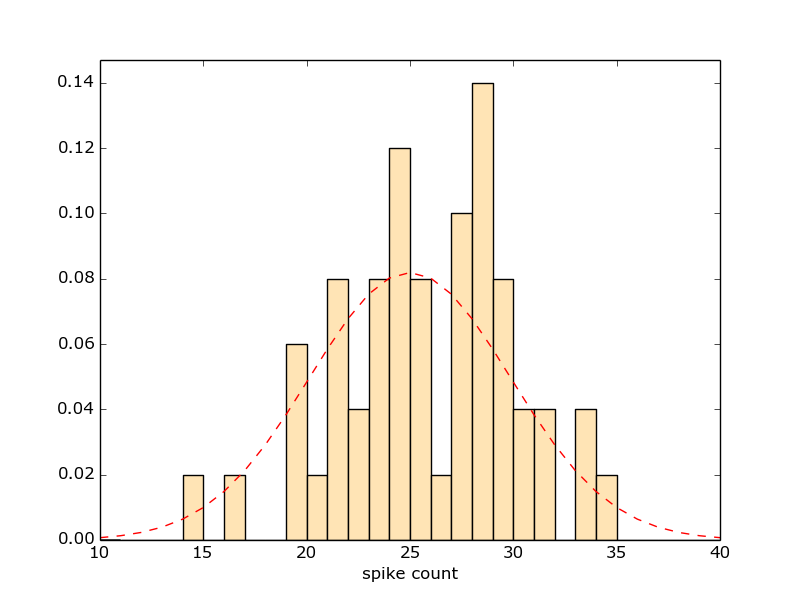
\includegraphics[width=0.7\linewidth]{stPoisson4}
  \caption{Histogram of total spike counts for 50 simulations}
\end{figure}

According to the central limit theorem, the distribution of spike counts here
(which is in fact the binomial distribution $B(500,0.05)$) can be
approximated by the normal distribution $\mathcal{N}(np,np(1-p))$ with 
$n = 500$ and $p = 0.05$ (the red dashed line in the figure). This can be more
or less seen above. However, the theoretical line doesn't fit yet very
well the simulation result. It's simply due to the fact that we have too few 
samples here to describe the distribution, but as we can see later the 
approximation itself works indeed pretty well.

We also plot the histogram of interspike intervals for the same set of spike
trains. This time the histogram follows an exponential distribution, as one
might expect (it's a property of the Poisson process).\\

\vspace*{-1em}
\begin{figure}[H]
  \centering
  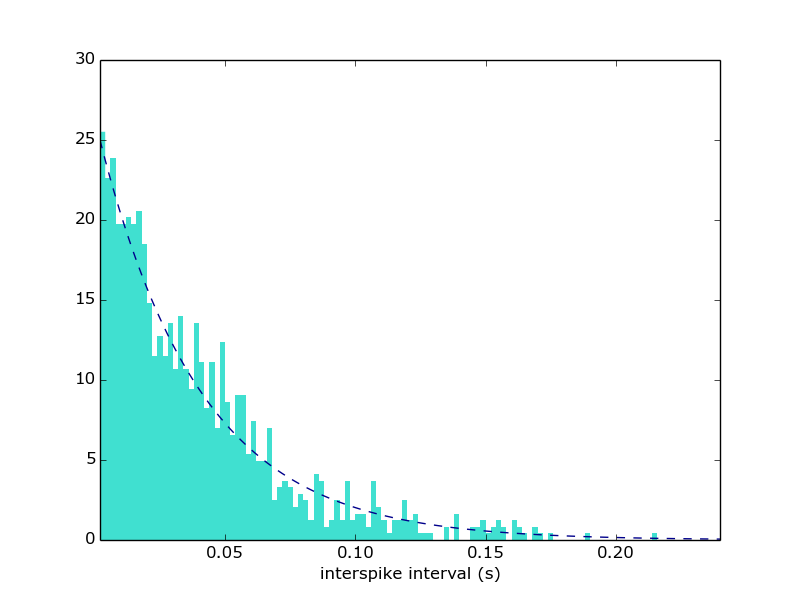
\includegraphics[width=0.7\linewidth]{stPoisson5}
  \caption{Histogram of interspike intervals counts for 50 simulations}
\end{figure}

\noindent
We redo the same plots but with now 500 simulated spike trains.

\vspace*{-1em}
\begin{figure}[H]
  \centering
  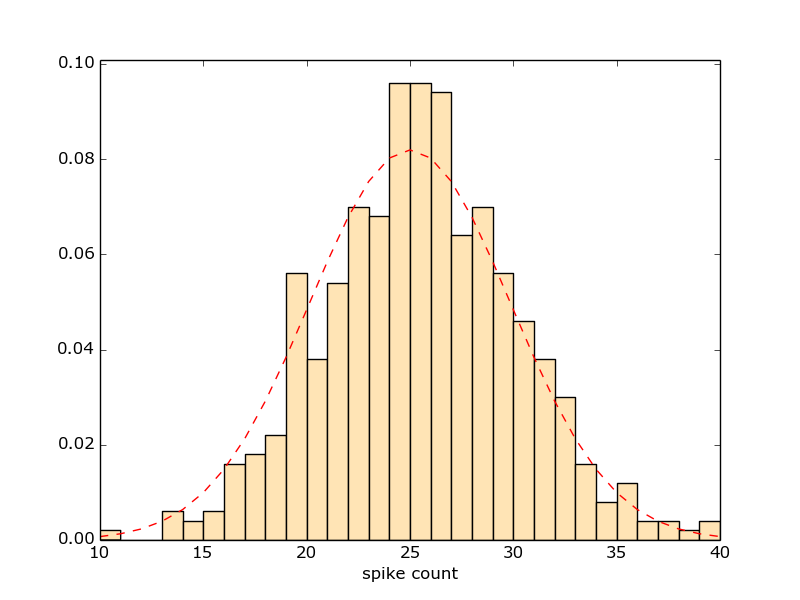
\includegraphics[width=0.7\linewidth]{stPoisson7}
  \caption{Histogram of total spike counts for 500 simulations}
\end{figure}

\begin{figure}[H]
  \centering
  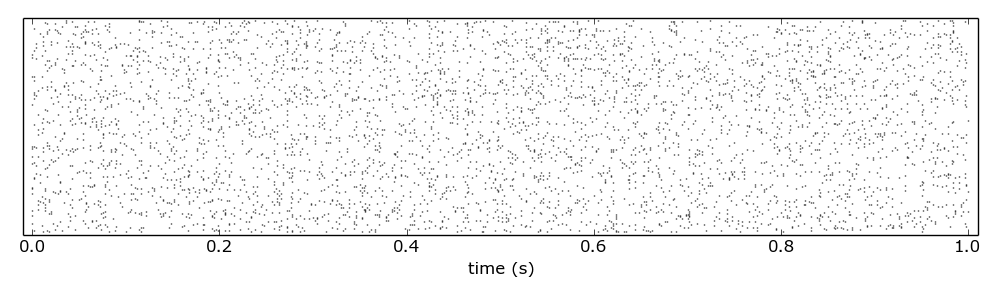
\includegraphics[width=0.9\linewidth]{stPoisson6}
  \caption{500 Poisson spike trains with firing rate 25 spikes/sec}
\end{figure}

\vspace*{-1em}
\begin{figure}[H]
  \centering
  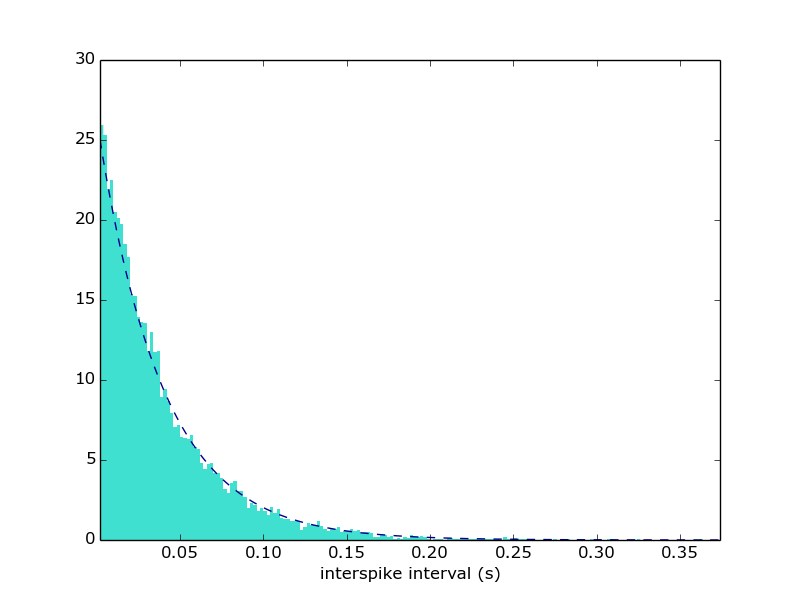
\includegraphics[width=0.7\linewidth]{stPoisson8}
  \caption{Histogram of interspike intervals counts for 500 simulations}
\end{figure}

\noindent
We observe that theoretical results fit much better.

\subsection{Analysis of spike trains}\label{subsec: anal_spikes}

Besides modeling the spike train generations, we'd also like to do some simple
analysis of real spike trains. We use thus the experimental data recorded from
a single neuron in the primary somatosensory cortex of a monkey that was
experiencing a vibratory stimulus. First we plot the spike trains for the
stimulus $f$ = 8.4 Hz into the graph below.

\begin{figure}[H]
  \centering
  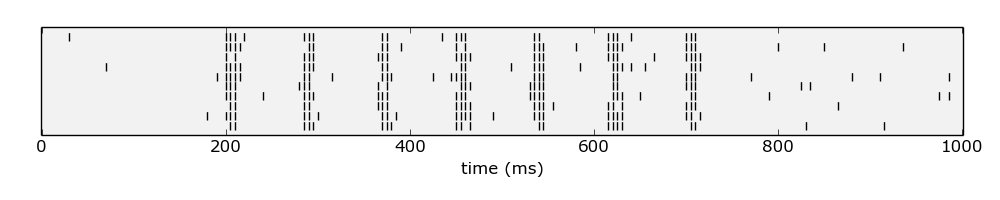
\includegraphics[width=\linewidth]{analSt1}
  \caption{Real spike trains recorded from a neuron in the primary
           somatosensory cortex of a monkey that was experiencing a vibratory 
           stimulus with $f$ = 8.4 z}
\end{figure}

Here we don't observe anymore the poisson process. Instead, we tend to see 
more spikes at some specific moments that are separated by some fixed length
time intervals. We now plot all the recorded spike trains into the same graph.
Alternate backgroud colors are meant to indicate different stimuli.

\begin{figure}[H]
  \centering
  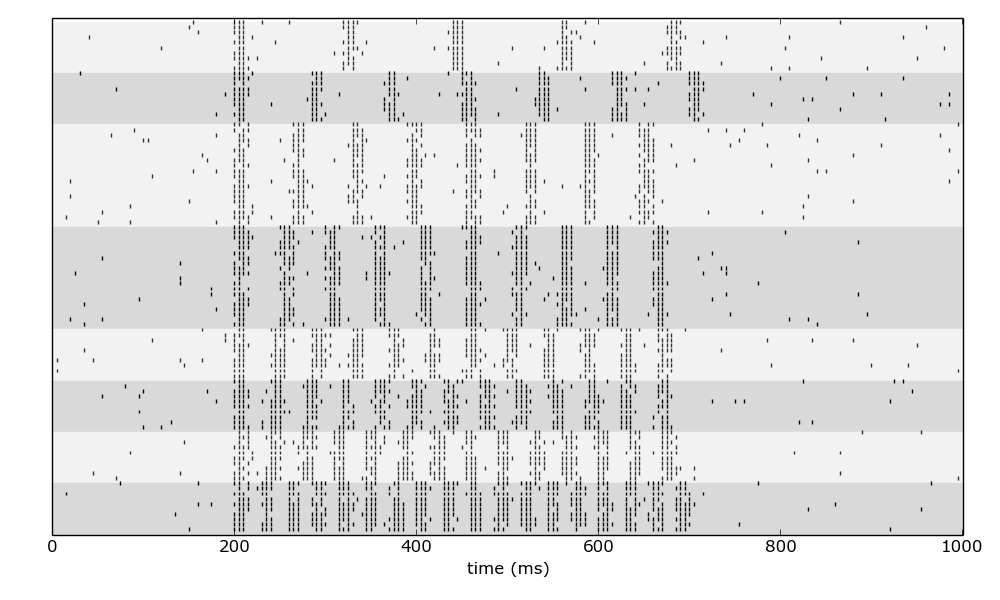
\includegraphics[width=\linewidth]{analSt2}
  \caption{Real spike trains recorded from a neuron in the primary
           somatosensory cortex of a monkey that was experiencing some 
           vibratory stimulus with different frequencies}
  \label{fig: real_spike_trains}
\end{figure}

The corresponding frequency for each dataset is not shown in the graph. In 
fact from top to bottom the frequency increases and we see that the seperating
time intervals also become shorter and the spike count augments. This shall be
even clearer if we give the exact numbers. The simulus is only present between
$t = 200$ ms and $t = 700$ ms. We compute the average spike count and the
standard deviation of spike counts for each stimulus.

\vspace{1em}
\begin{table}[h]
  \tabcolsep = 11pt
  \caption
    {Mean values and standard deviations of spike counts for different stimuli}
  \label{tab: meanstd}
  \begin{tabular*}{\linewidth}{>{\it}lcccccccc}
    \toprule
    Frequency (Hz) & 8.4 & 12 & 15.7 & 19.6 & 23.6 & 25.9 & 27.7 & 35 \\ 
    Average spike count $m$ 
    & 16.5 & 19.2 & 23.6 & 29.9 & 35.6 & 39.5 & 41.8 & 52.3 \\
    Standard deviation $\sigma$ 
    & 1.80 & 1.47 & 1.96 & 1.58 & 2.50 & 5.94 & 1.89 & 3.26 \\
    \bottomrule
  \end{tabular*}
\end{table}
\vspace{0.4em}

Sure when the frequency gets higher, the average spike count increase as well.
We plot also the tuing curve of the neuron. 

\begin{figure}[H]
  \centering
  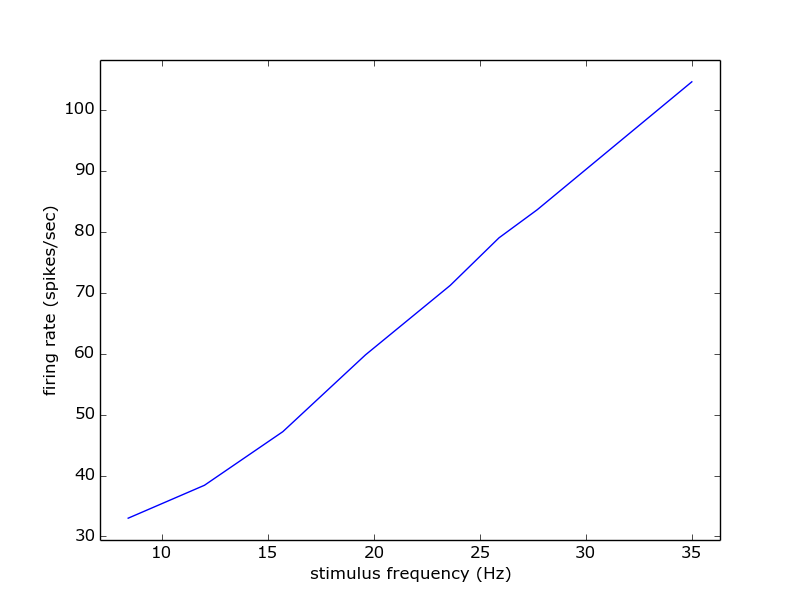
\includegraphics[width=0.7\linewidth]{analSt3}
  \caption{Tunning curve of the neuron}
\end{figure}

The relation between the average firing rate and the stimulus frequency is
almost linear. We may also want to show that the mean value and the standad
deviation of spike counts are positively correlated and even try to find an
explicit relation between these two quantities (for example in the case when 
the spike count is sampled from some poisson distributions we have 
$\mu = \sigma^2$). However, with the values given in \autoref{tab: meanstd}, 
we can not easily draw a conclusion.


\section{Leaky Integrate-And-Fire Model}

\subsection{Model description}

Let's look more closely at how spikes are generated in a cell from a 
biophysical point of view. In a biologically detailed model, we might need 
to take into account the topology of the neuronal tree and at the same time
establish a model for each basic component of the neuron. Finally, the 
interactions between different components should also be simulated. 
It can be very complicated and thus, we'll consider a much more 
simplified model here that however still fits quite well experimental data.

In the leaky integrate-and-fire (LIF) model, the whole neuron is collapsed to
a single point. The cell membrane acts like a RC circuit and the relationship
between the output voltage $V(t)$ and the input current $I(t)$ is therefore
given by

\begin{equation}
  \label{eq: LIF}
  C\frac{dV(t)}{dt} = g_L(E_L - V(t)) + I(t)
\end{equation}

\noindent
where $C$ is the membrane capacitance, $g_L = 1/R$ is the conductance of the
membrane that contributes to the leak term and $E_L$ is the reversal
potential. 
This equation can be solved numerically using the Euler method, that is 

\begin{equation}
  V(t + \Delta t) = V(t) + \frac{dV(t)}{dt}\Delta t
\end{equation}

\noindent
for a small $\Delta t$. Otherwise, we can also solve the equation analytically
and get

\begin{equation}
  \label{eq: LIF_sol}
  V(t) = (V(0)-E_L)\exp(-\frac{t}{\tau_m}) + E_L + \frac{1}{C}
  \int_0^t\exp(-\frac{s}{\tau_m})I(t-s)ds
\end{equation}

\noindent
where $\tau_m = RC$ is the membrane time constant. The analytic solution is
useful when the integral has an explicit expression since the result is
generally of better precision and the computation gets also faster.

The spiking events are then characterized by a firing time $t$ that is defined
by a threshold criterion. In other words, every time when the membrane voltage
$V$ reaches a certain threshold $V_{th}$, the neuron emits an action potential
and $V$ is reset to $E_L$.

\subsection{constant stimulation}

Let us start by studying a simple example here. Suppose that the
integrate-and-fire neuron is stimulated by a constant input current 
$I(t) = I_0$. We compute first the solution of \eqref{eq: LIF} using the Euler
method. For the parameters, we fix $C = 1$nF, $g_L = 0.1 \mu$S, $E_L = -70$
mV, $V(0) = E_L$, $I_0 = 1$ nA and $\Delta t = 1$ ms. We run the simulation
until $t = 100$ ms.

\vspace{-1em}
\begin{figure}[H]
  \centering
  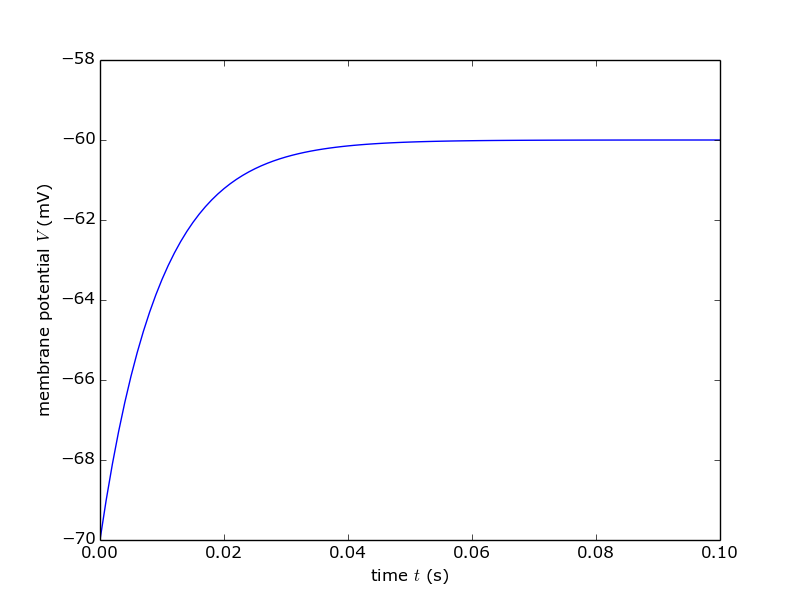
\includegraphics[width=0.7\linewidth]{LIF1}
  \caption{LIF model without spiking mechanism 
           with constant input current $I = 1$ nA}
\end{figure}

We observe an exponential rise to a limit value $V_{\infty} = E_L + RI_0$. In
\autoref{fig: LIF_cst_Is}, we compare the results of several different input 
currents. When $I$ is higher, $V$ climbs faster at the beginning and the final
value is as well higher, though, the characteristic time doesn't change. 

We may also be interested in the effect of $\Delta t$. From a mathematical
point of view, the smaller is $\Delta t$, the better. In fact, we can see in
\autoref{fig: LIF_cst_dts} that when the stepwidth increases, the numerical
error with the real value of $V$ gets equally larger (though sure, we can
never represent the ``real" value in a figure, but say, intuitively). 
However, more computations are also required when $\Delta t$ gets smaller, a
trade-off needs to be found. It's also shown in the figure that
the two curves $\Delta t = 1$ ms and $\Delta t = 0.1$ ms are close,
which means that $\Delta t = 1$ ms is already quite a sensible choice that 
allows us to have a good precision of $V$.

\vspace{-1em}
\begin{figure}[H]
  \centering
  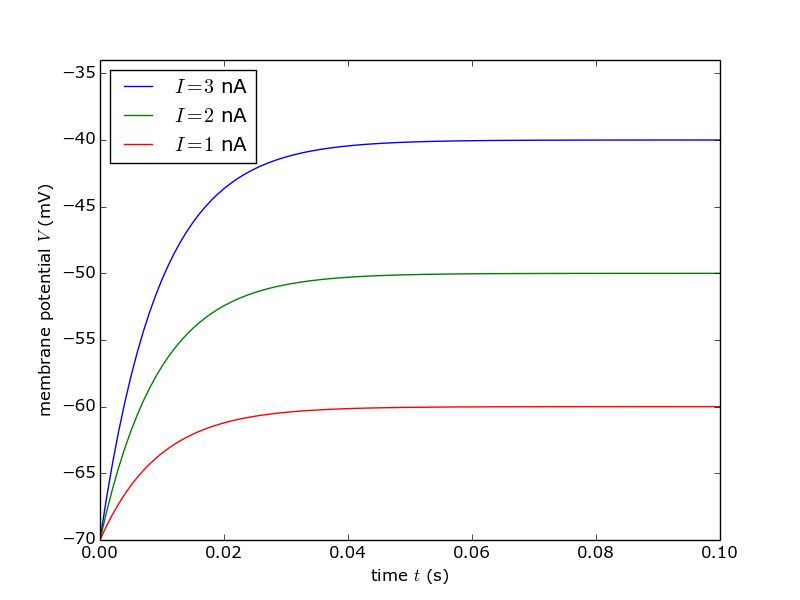
\includegraphics[width=0.7\linewidth]{LIF2}
  \caption{Different constant input currents}
  \label{fig: LIF_cst_Is}
\end{figure}

\vspace{-1em}
\begin{figure}[H]
  \centering
  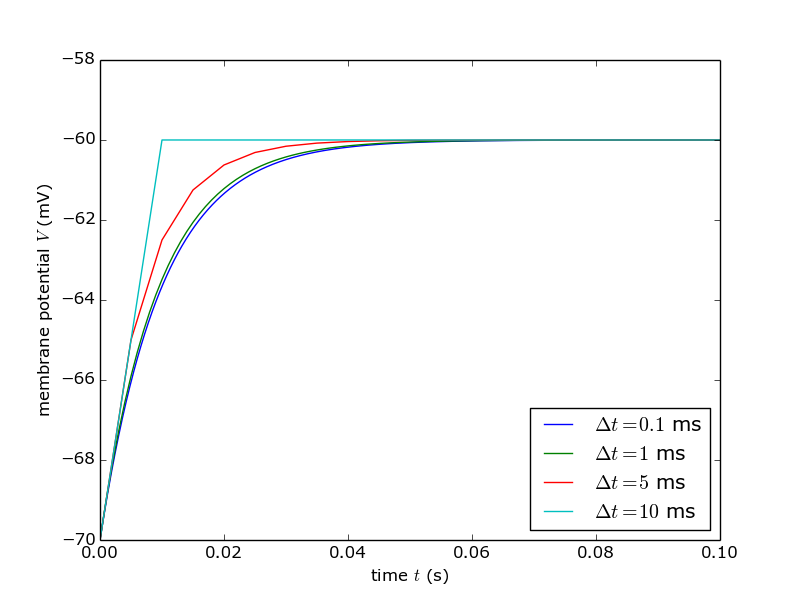
\includegraphics[width=0.7\linewidth]{LIF3}
  \caption{Effect of $\Delta t$ ($I = 1$ nA)}
  \label{fig: LIF_cst_dts}
\end{figure}

By using the equation \eqref{eq: LIF_sol} we know that in this case the
analytic solution is given by

\begin{equation}
  \label{eq: LIF_cst_sol}
  V(t) = V_{\infty} + (V(0) - V_{\infty})\exp(-\frac{t}{\tau_m}).
\end{equation}

\noindent
The explicit expression allows us to verify the validity of the numerical
approach. We compare thereby the plots of the two solutions under the condition
$I = 1$ nA. For the numerical part, we use $\Delta t = 1$ ms. As shown in
\autoref{fig: LIF_comp_anal_nume}, the two curves are similar and with what is
mentioned above, if we decrease $\Delta t$, we can approach the analytic
solution. (This may be confusing, but the plot of the analytic solution in the
graph isn't either the true value of $V$ since time is not continue in a
computer. In effect, the plot is done by using a time bin of $1$ ms.)

\vspace{-1em}
\begin{figure}[H]
  \centering
  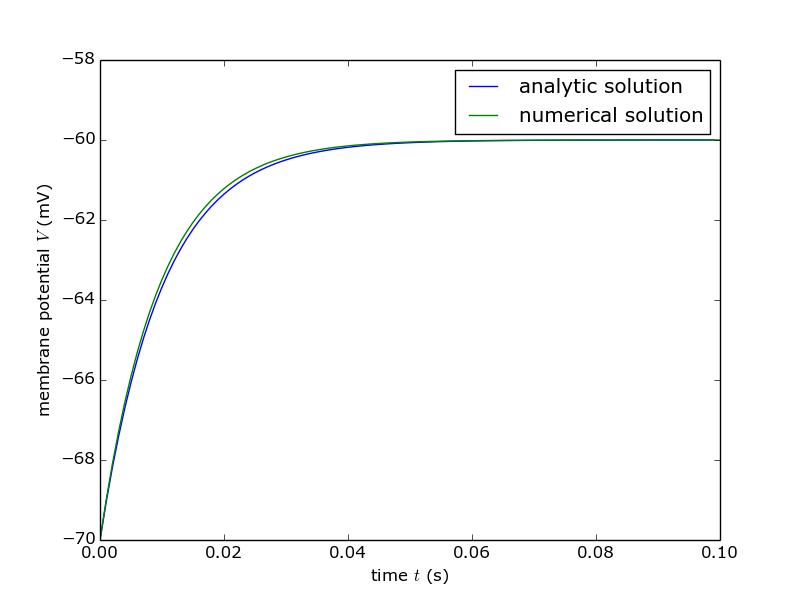
\includegraphics[width=0.7\linewidth]{LIF4}
  \caption{Comparison of analytic and numerical solutions ($I = 1$ nA)}
  \label{fig: LIF_comp_anal_nume}
\end{figure}

We now equip the cell with the simple spiking mechanism as described before.
We choose $V_{th} = -63$ mV and vary the value of input current. The results
are plotted seperately in oreder to get a better view. Here we use 
$\Delta t = 0.1$ ms. We can imagine that with a larger stepwidth, we're not
able to have a good precision of spike moments.

\vspace{-1em}
\begin{figure}[H]
  \centering
  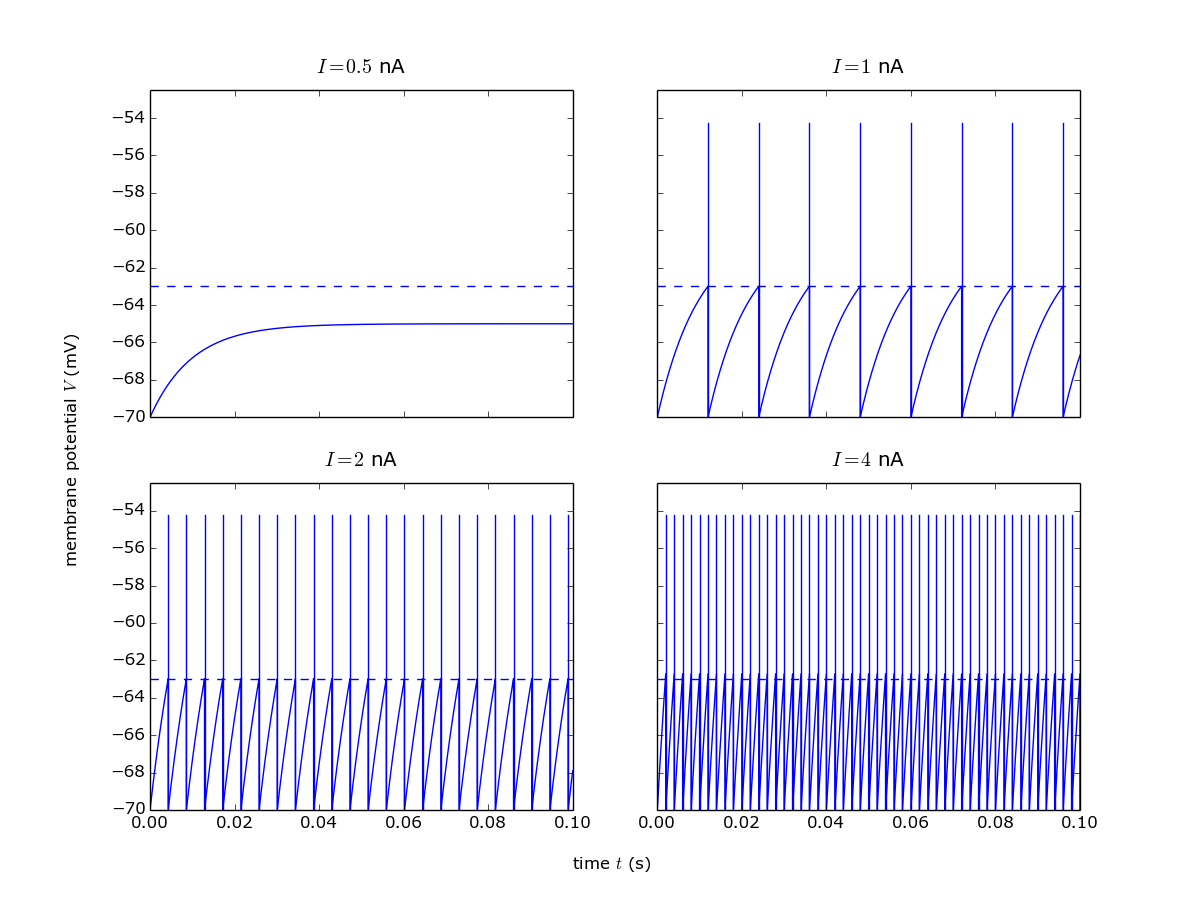
\includegraphics[width=1\linewidth]{LIF5}
  \caption{LIF model with constant input current}
\end{figure}

We get more spikes within the first $t = 100$ ms when $I$ augments, which
means that the firing rate increases. Nevertheless, smaller $\Delta t$ is
needed to capture a higher firing rate. This can be more or less seen from the
case $I = 4$ nA where we have the feeling that spikes are not immediately
generated after the threshold is reached. On the other hand, when $I = 0.5$ nA,
no spikes are emitted. As a matter of fact, we need to have 
$V_{\infty} > V_{th}$ for the neuron to fire. It means that the condition for
$I$ is $I > g_L(V_{th}-E_L)$. The exact firing rate can also be computed under
this hypothesis, we first compute the time $T$ that it takes for $V$ to reach 
the threshold $V_{th}$ from $E_L$, and then we have $f_{firing} = T^{-1}$. 
The explicit formula is

\begin{equation}
  \label{eq: LIF_firing}
  f_{firing} = (\tau_m \log(\frac{E_L-V_{\infty}}{V_{th}-V_{\infty}}))^{-1}
\end{equation}

In the figure below we plot the tunning curve of the neuron, i.e. the number 
of spikes within 100 ms as a function of the input current $I$. The two curves
are acquired respectivly by using \eqref{eq: LIF_firing} and by simulating
directly the integrate-and-fire mechanism.

\vspace{-1em}
\begin{figure}[H]
  \centering
  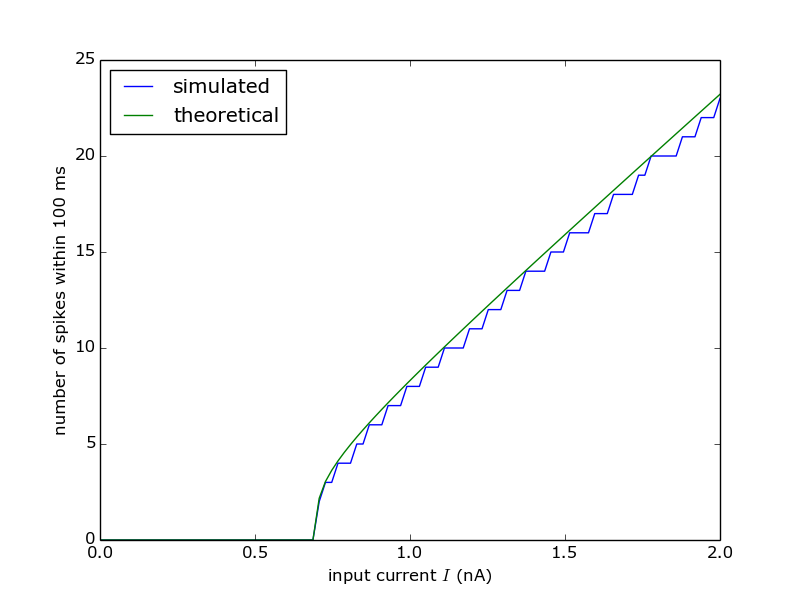
\includegraphics[width=0.7\linewidth]{LIF6}
  \caption{Tunning curve of the LIF neuron when $I$ is constant}
\end{figure}

With the given parameter, $g_L(V_{th}-E_L) = 0.7$ nA. We observe in the graph
the neuron starts firing indeed at about $I = 0.7$ nA. The curve obtained by
the simulation approximates quite well the theoretical curve. The jagged shape
comes from the fact that in the simulation, $V$ is reset to $E_L$ every $k$ 
time bins for some integer $k$, so the number of spikes within 100 ms is then
$\lfloor 1000/k \rfloor$ (with $\Delta t = 0.1$ ms).


\subsection{Refractory period and noise term}

For the moment being the stimulus is always a constant current, but we'd like
to add some new elements in the model to make it more realistic. The first 
step is to introduce a refractory period. A simple idea is to fix $V(t) = E_L$ 
for a small amount of time $\Delta$ after each spike, and the differential
equation comes into play only after this period. Under this new hypothesis, 
we plot again the evolution of the membrane voltage $V$. Here $\Delta = 3$ ms.

\vspace{-1em}
\begin{figure}[H]
  \centering
  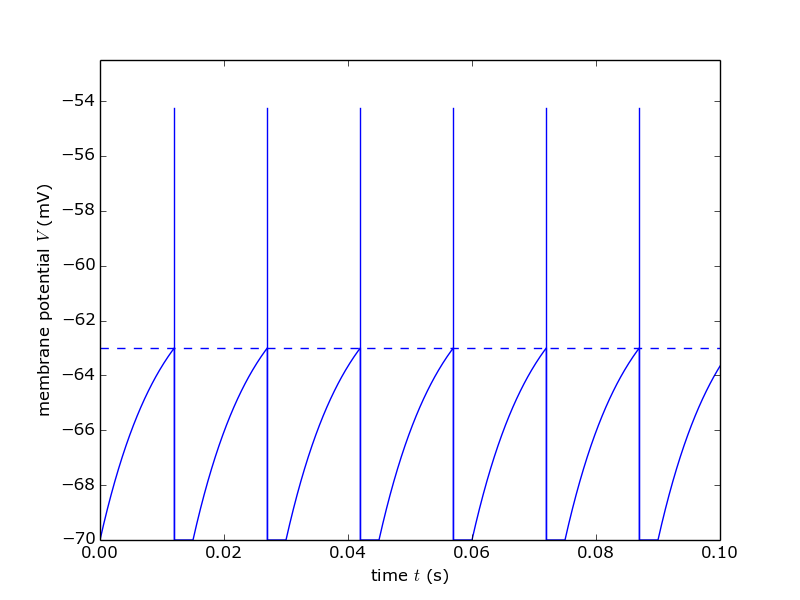
\includegraphics[width=0.7\linewidth]{LIF7}
  \caption{LIF neuron with refractory period ($I=1$ nA)}
\end{figure}

\noindent
The new firing rate becomes 

\begin{equation}
  \label{eq: LIF_ref_firing}
  f_{firing} = (\Delta +
                \tau_m \log(\frac{E_L-V_{\infty}}{V_{th}-V_{\infty}}))^{-1}.
\end{equation}

\noindent
It's more realistic since it admits a supremum. We compare the tunning curve
of the original model and the model with the refractory period. Due to the
reason that is explained before (some innate constraints of the simulated
result), we plot the curves using the analytic formulas 
\eqref{eq: LIF_firing} and \eqref{eq: LIF_ref_firing}, which allows us to
have a greater variation of $I$ and the difference between two models becomes
also clearer.

\vspace{-1em}
\begin{figure}[H]
  \centering
  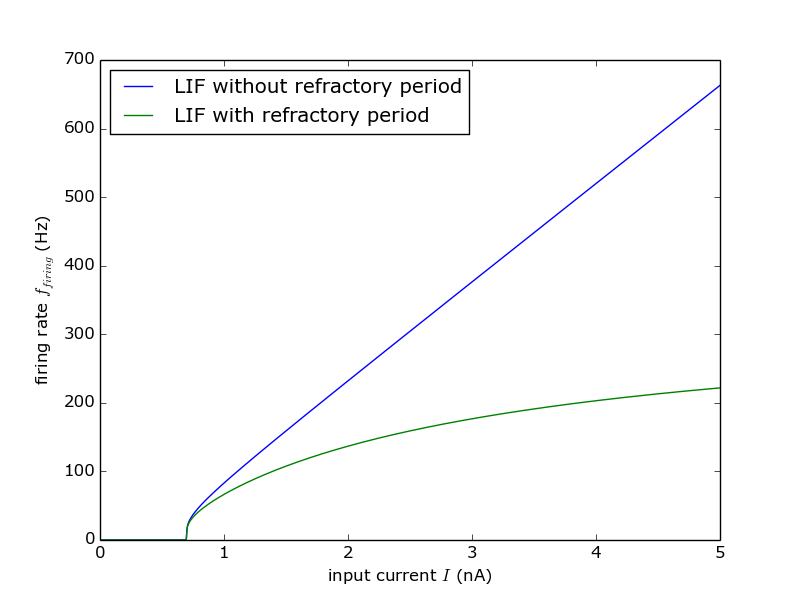
\includegraphics[width=0.7\linewidth]{LIF8}
  \caption{Tunning curve of the LIF model with and 
           without refractory period ($I$ constant)}
\end{figure}

\newpage
The second step is to add a white noise term $\eta(t)$ in the simulaton, so
the differential equation turns into

\begin{equation}
  C\frac{dV(t)}{dt} = g_L(E_L-V(t)) + I(t) + \sigma\eta(t)
\end{equation}

\noindent
where $\sigma$ is the magnitude of the noise. To compute the solution, we use
the Euler-Maruyama method

\begin{equation}
  \label{eq: Euler-Maruyama}
  V(t + \Delta t) = V(t) + \frac{dV(t)}{dt}\Delta t 
  + \sigma\tilde{\eta}(t)\sqrt{\Delta t}.
\end{equation}

\noindent
Since we want to add a Gaussian white noise term here, $\tilde{\eta}(t)$ is
drawn randomly from a standard Gaussian distribution (sure $\eta(t)$ and
$\tilde{\eta}(t)$ are related). To understand where the square root comes 
from, roughly speaking, when we add a noise term, we want to add a variance
but not a mean to the random variable. If we write directly in a discret form,
we may have something like
($\Delta t$ is fixed and we have some discret time moments 
$t_0, t_1, ..., t_n, t_{n+1}, ...$)

\begin{equation}
  X_{n+1} = X_n + a(X_n)\Delta t + b(X_n) \Delta W_n
\end{equation}

\noindent
where $X$ is the stochastic process that we are interested in and 
$\Delta W_n$ contributes to the noise term ($W$ is also some stochastic 
process but we'll not go into detail here). Then what we want to get is 
in fact

\begin{align}
  \mathrm{E}\thinspace[\Delta X_n \thinspace|\thinspace X_n] & 
  = a(X_n)\Delta t,\\
  \mathrm{Var}\thinspace(\Delta X_n \thinspace|\thinspace X_n) & 
  = b(X_n)^2\Delta t,
\end{align}

\noindent
which means that $\Delta W_n$ is of variance $\Delta t$, and if we put this
back in the equation \eqref{eq: Euler-Maruyama}, it corresponds to the term
$\tilde{\eta}(t)\sqrt{\Delta t}$. We'll run this model for the choice 
$\sigma = 1$ $\mathrm{mV\cdot ms^{-1/2}}$.

\vspace{-1em}
\begin{figure}[H]
  \centering
  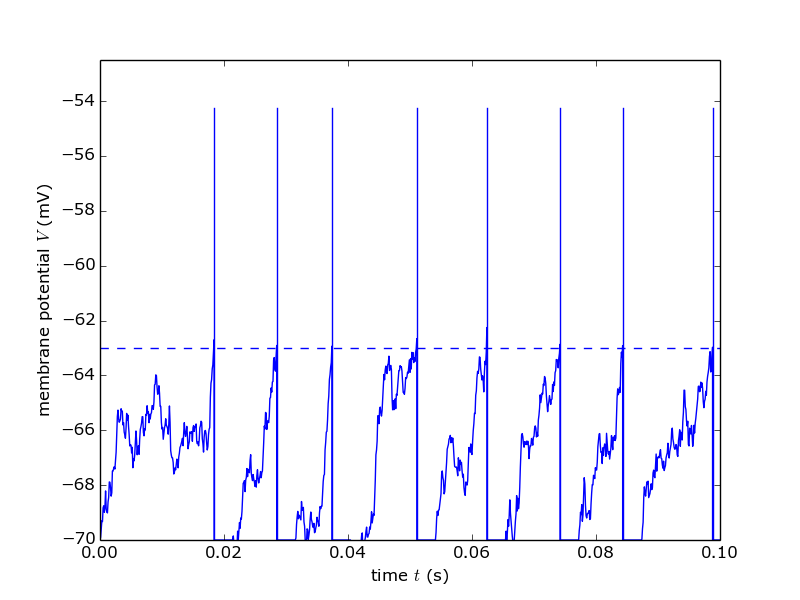
\includegraphics[width=0.7\linewidth]{LIF9}
  \caption{LIF neuron with noise and refractory period ($I=1$ nA)}
\end{figure}

Now we have introduced refractory period and noise in our model, we plot
the generated spike trains with varying noise levels in 
\autoref{fig: LIF_noise_trains}. We notice that when
$\sigma$ is smaller, spike trains are more regular, which is quite sensible,
but what is also interesting is to observe that we tend to get more spikes
when $\sigma$ gets larger ($V$ oscillates with greater amplitude).

\begin{figure}[H]
  \centering
  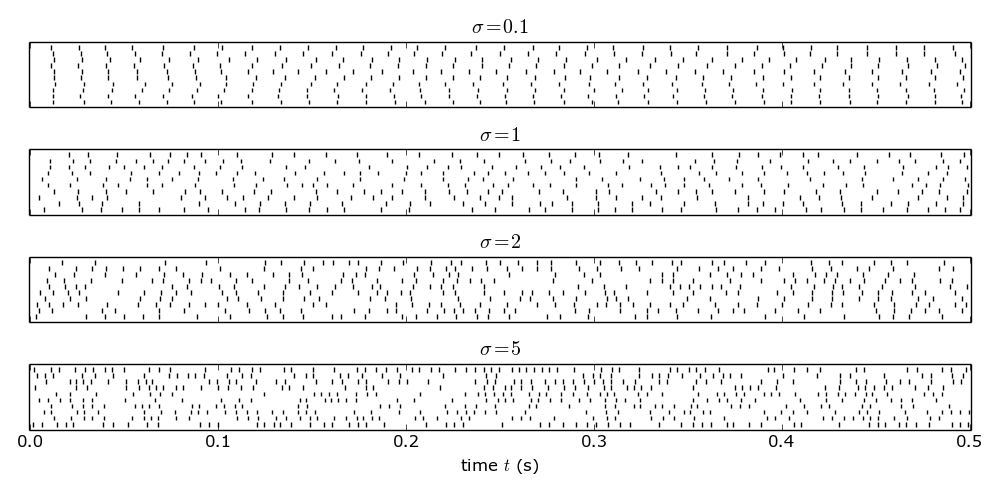
\includegraphics[width=0.9\linewidth]{LIF10}
  \caption{Spike trains generated by the above model with cosntant input
           current $I = 1$ nA and varying $\sigma$ (in 
           $\mathrm{mV\cdot ms^{-1/2}}$)}
  \label{fig: LIF_noise_trains}
\end{figure}


\subsection{Compare with experimental data}

Our goal is now to generate spike trains that we have seen in 
\ref{subsec: anal_spikes}. We first obeserve that we get more spikes at some
specific times while during the rest of the experiment, spikes are quite 
sparse and may just come from neuronal noise. Let us say that between some 
$\tilde{t}$ and $\tilde{t} + \Delta\tilde{t}$ we tend to observe more spikes 
(in a spike train there are several different $\tilde{t}$). 
Next, we notice that such a $\tilde{t}$ appears exactly with the frequncy $f$,
while $\Delta\tilde{t}$ seems to be independant of $f$. From the data, 
$\Delta\tilde{t} \sim 14$ ms. We can thus assume that $I$ has some 
constant value during such a period and is zero otherwise, just like what 
is shown below (with $f = 20$ Hz).

\vspace{-1em}
\begin{figure}[H]
  \centering
  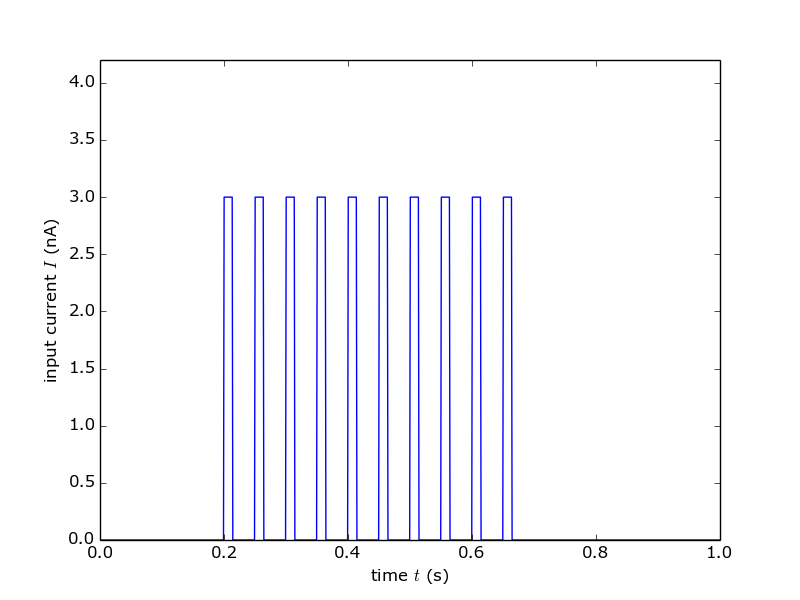
\includegraphics[width=0.7\linewidth]{LIF11}
  \caption{An assumption of the input current that can generate 
           spike trains shown in \autoref{fig: real_spike_trains}}
\end{figure}

\newpage
Here the constant value of $I$ is 3 nA. It's a little higher than before. 
In fact, we observe that spikes are quite dense at these specific moments 
$\tilde{t}$, which suggests a larger value of $I$. With these input currents,
the spike trains generated by the model are plotted below
(we use the same parameters for the LIF neuron except 
$\sigma = 1.3$ $\mathrm{mV\cdot ms^{-1/2}}$). 
As before from top to bottom the frequency increases. The result that we 
obtain here is very similar to the experimental data.

\begin{figure}[H]
  \centering
  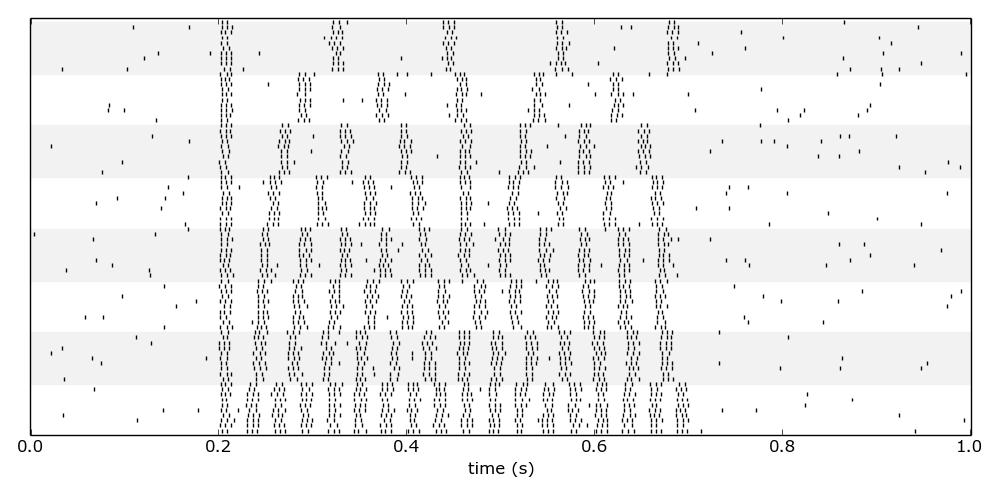
\includegraphics[width=0.9\linewidth]{LIF12}
  \caption{Some spike trains generated by the LIF model that are comparable
           with \autoref{fig: real_spike_trains}}
  \label{fig: sim_spike_trains}
\end{figure}

\subsection{Sinusoidal stimuli}

We'll come back to the initial model with neither refractory period nor 
noise term, but we'll now be interested in time-dependent stimuli.
The input current is of the form 

\begin{equation}
  I(t) = 1 + \sin(2\pi ft)
\end{equation}

\noindent
where $f$ is the frequency of the stimulus, expressed in Hz. For the sake of 
simplicity, we'll ignore all the electrical units (for $I$, $V$, etc ...) 
in this part of simulation and we say that $E_L = 0$ and $V_{th} = 1$.  
We use a discretization of time in time bins of width 0.1 ms and we'll first 
plot three different stimuli with frequencies 1 Hz, 5 Hz and 40 Hz for 1 
second duration. The result is shown in \autoref{fig: sin_I}.

A stimulus of frequency $f$ is characterized by a smooth repetive oscillation
of amplitude 1 and period $T = f^{-1}$. To see how our neuron responds to
this kind of stimuli, we'll first forget the threshold mechanism and 
solve just the equation \eqref{eq: LIF} using the Euler method. 
For the membrane parameters, we take $R = 1$ and $\tau_m = 0.1$ s, and we plot
the evolution of the membrane potential in response to the current of 
frequency 1 Hz in \autoref{fig: LIF_sin}.

\vspace{-1em}
\begin{figure}[H]
  \centering
  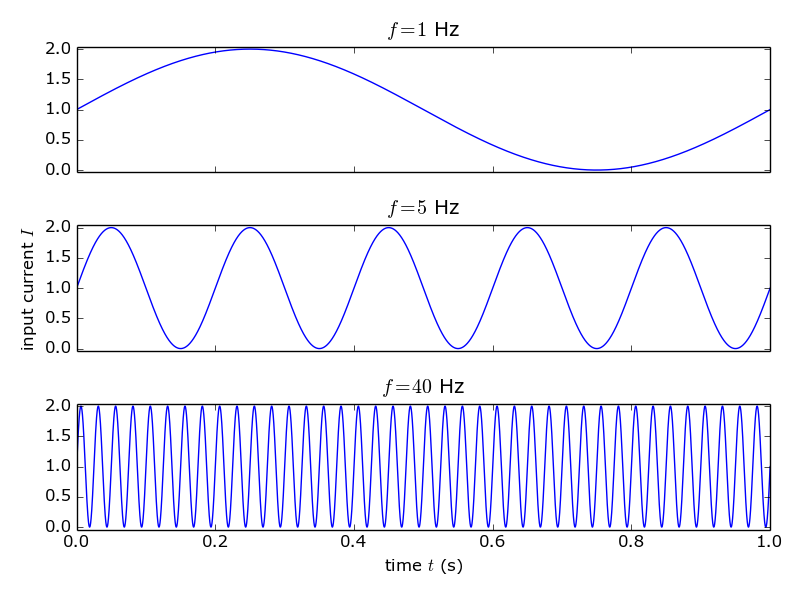
\includegraphics[width=0.7\linewidth]{LIFSin1}
  \caption{Sinusoidal input currents}
  \label{fig: sin_I}
\end{figure}

\vspace{-1em}
\begin{figure}[H]
  \centering
  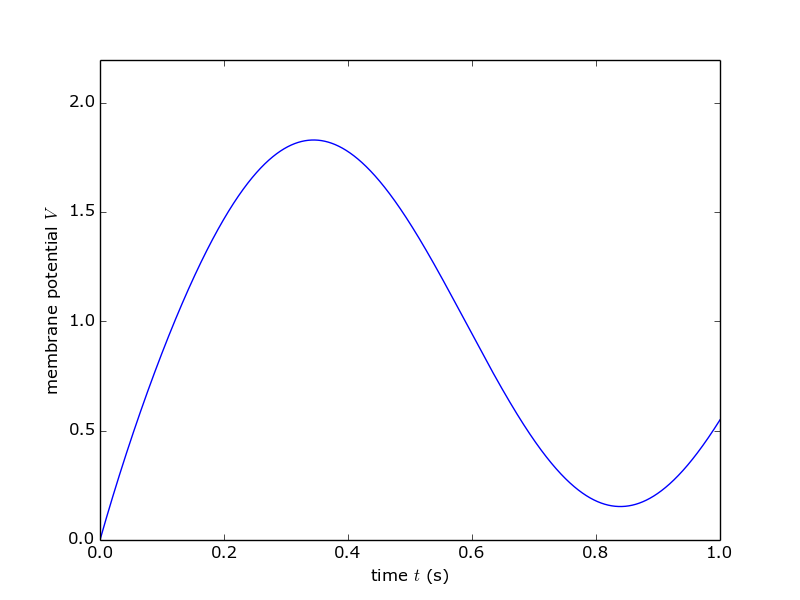
\includegraphics[width=0.7\linewidth]{LIFSin2}
  \caption{LIF neuron without spiking mechanism in response to 
           sinusoidal stimulus of frequency 1 Hz}
  \label{fig: LIF_sin}
\end{figure}

After comparing the plots of the input current $I$ and the output voltage $V$,
it seems there will be more spikes near the crest of the input current, 
though there may be a certain delay between $V$ and $I$. In effect, by using
\eqref{eq: LIF_sol}, we can deduce the exact solution 

\begin{equation}
  \label{eq: LIF_sin_sol}
  V(t) = (V(0) -E_L - R + \frac{2\pi f\tau_mR}{4\pi^2f^2\tau_m^2 + 1})
         \exp(-\frac{t}{\tau_m}) + E_L + R
         + \frac{R\sin(2\pi ft-\phi)}{\sqrt{4\pi^2f^2\tau_m^2+1}}
\end{equation}

\noindent
where $\phi = \arctan(2\pi f\tau_m)$ is the phase delay of $V$ with respect
to $I$. One may notice that the above equation is not homogeneous. 
It's simply because the unit of $I$ is neglected here. When $t$ is large 
enough, the exponentially decreasing term can be ignored (transitional phase),
and knowing that $V(0) = E_L = 0$ and $R = 1$, we write

\begin{equation}
  V(t) = 1 + \frac{\sin(2\pi ft-\phi)}{\sqrt{4\pi^2f^2\tau_m^2+1}}.
\end{equation}

\noindent
This should justify our intuition about the shape of the $V$.

We insert again the threshold mechanism and we plot the reponse of the LIF
neuron to the three input currents defined earlier.

\vspace{-1em}
\begin{figure}[H]
  \centering
  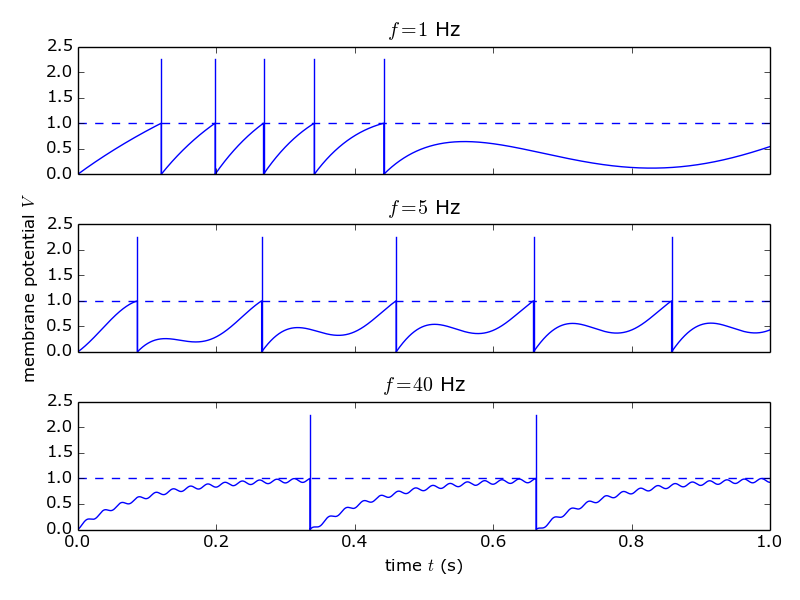
\includegraphics[width=0.7\linewidth]{LIFSin3}
  \caption{LIF neuron in response to sinusoidal stimuli}
\end{figure}

These curves are quite interesting. For the first input current, as predicted,
several spikes are generated near the crest of $I$, and for the second
input current, we get one spike for each period. Finally, in the case 
where $f = 40$ Hz, the neuron's response seems more particular: the integral
curve is very similar to what we have seen before when the stimulus is 
constant. By looking at the analytic solution \eqref{eq: LIF_sin_sol}, we
may have a simple idea of what's happening here. As a matter of fact, when 
$f$ tends to infinity, the two terms that depend on $f$ decrease to 0
and we find again the equation \eqref{eq: LIF_cst_sol} which is the solution
of $V$ for an input current that is constant.

From this analytic solution we also see that the characteristic time
plays an important role here. Intuitively, in our case, $\tau_m = 0.1$ ms
is too long with respect to a 40 Hz oscillation, thus the neuron is not able
to integrate enough voltage to fire a spike in a single period of the 
stimulus. Nonetheless, the response can be different if we reduce $\tau_m$.
For instance, in \autoref{fig: LIF_sin_small_tau_m}, the characteristic time
is reduced to 0.01 s, and we see that the neuron gets sort of more sensitive 
when $\tau_m$ decreases. 

Let us change $\tau_m$ back to 0.1 s and plot the firing rate of the neuron
as a function of the frequency of the input (\autoref{fig: LIF_sin_tunning}). 
The firing rate is computed by simulating the  model until $t = 25$ s and 
then devide the total number of spikes we get by 25.

\vspace{-1em}
\begin{figure}[H]
  \centering
  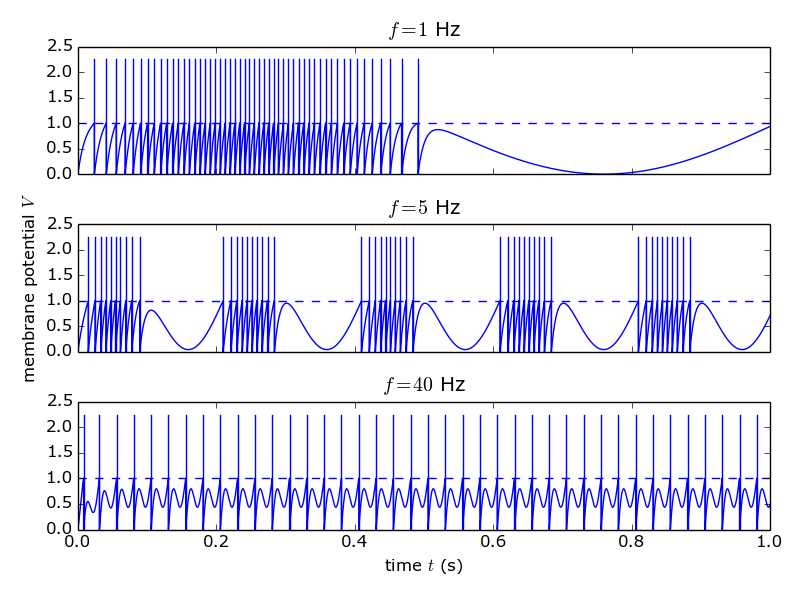
\includegraphics[width=0.7\linewidth]{LIFSin4}
  \caption{LIF neuron in response to sinusoidal stimuli, $\tau_m = 0.01$ s}
  \label{fig: LIF_sin_small_tau_m}
\end{figure}

\vspace{-1em}
\begin{figure}[H]
  \centering
  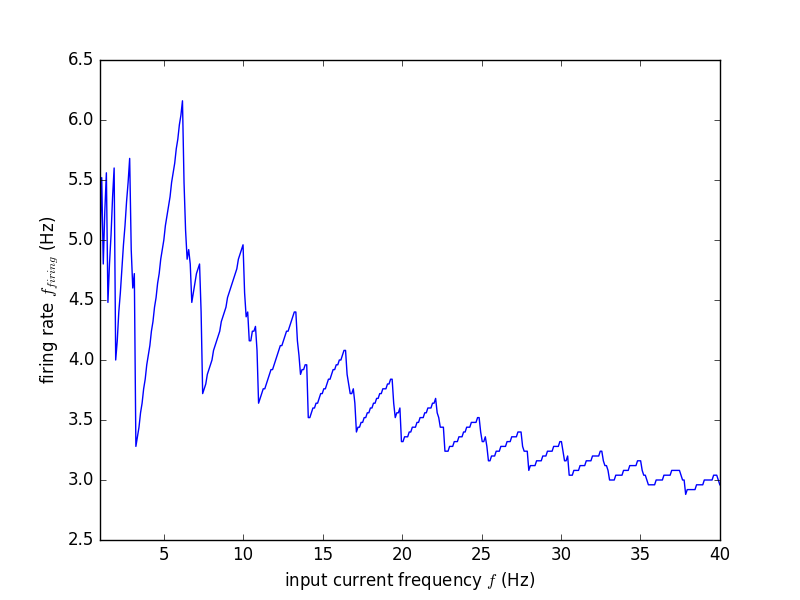
\includegraphics[width=0.7\linewidth]{LIFSin5}
  \caption{Tunning curve of the LIF neuron when $I$ is sinusoidal}
  \label{fig: LIF_sin_tunning}
\end{figure}

It seems that we observe some exponential decay but with oscillations of
great amplitude, not very sure. The form of the curve can be explained by 
studying in more detail the equation \eqref{eq: LIF_sin_sol}, mainly by
looking at the effect of the sinusoidal term and the exponential term,
but here we're rather insterested in the question that if the frequency $f$
of the input current can be coded in this curve. Given some firing rate, we
have a range of different possible input frequencies, so the firing rate of
this single neuron may not be explicitly coding $f$, but it can still gives
us information about it which can probably be used later to determine $f$
on a larger scale.

Besides just looking at the neurons's firing rate, we ask if the temporal fine
strucutre of the spike train is also able to code the stimulus frequency in
some way. We plot thus the spike trains that result from different $f$ in 
the \autoref{fig: spike_train_sin}. From top to bottom the frequencies are 
respectively 1, 2, 5, 10, 20, 40 and 100 Hz.

\begin{figure}[H]
  \centering
  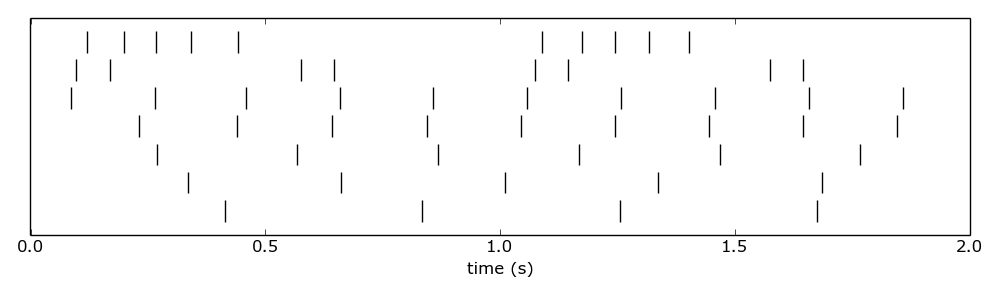
\includegraphics[width=0.9\linewidth]{LIFSin6}
  \caption{Spike trains for sinusoidal input currents}
  \label{fig: spike_train_sin}
\end{figure}

We see that spike trains seem to be periodic. We suppose then the period
$T_r$ of the neuronal response is somehow related to the input current 
frequency $f$. However, we need to find an algorithm to compute $T_r$.
A priori, we're not aware of the number of spikes in each period. 
We don't have necessarily the same local structures and this can become even 
more complex if we take into account neuronal noise. It's not obvious that 
we are able to compute $T_r$ directly from the data at hand.

Since a spike train is just a sequence of 0 and 1, which is not suitable 
for signal processing, what I decide to do here is first to conduct a 
convolution of the spike train with a hann window of size 0.3 s. 
Next, we perform a fourier transform and have now the information about 
the frequency spectrum of the data (as shown in \autoref{fig: LIF_freq_spec}, 
with $f = 20$ Hz). The last thing to do is to find the frequency 
$f_r = T_r^{-1}$ that has the greatest amplitude in the frequency domain 
(we exclude the constant component). We plot then $f_r$ as against $f$ in
\autoref{fig: LIF_f_fr}.

\vspace{-1em}
\begin{figure}[H]
  \centering
  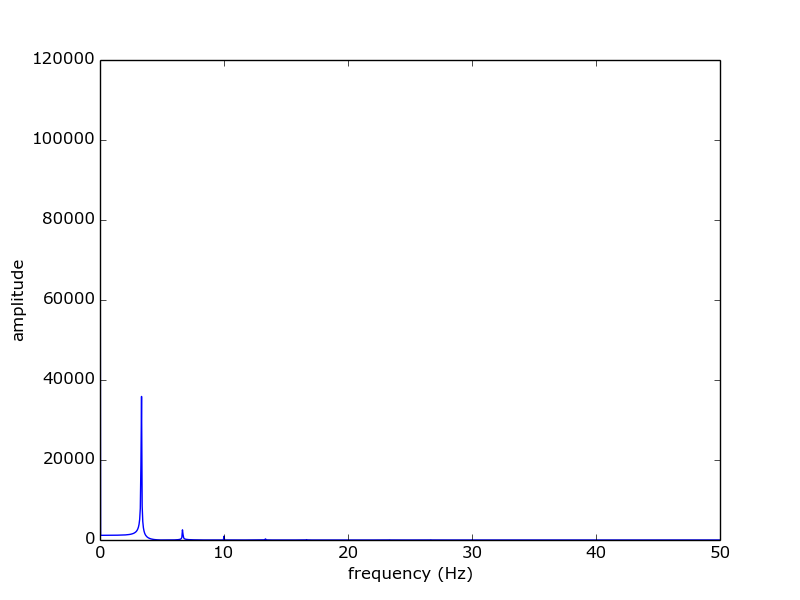
\includegraphics[width=0.7\linewidth]{LIFSin7}
  \caption{Frequency spectrum of the neuronal response when 
           the input current frequncy is 20 Hz}
  \label{fig: LIF_freq_spec}
\end{figure}

\vspace{-1em}
\begin{figure}[H]
  \centering
  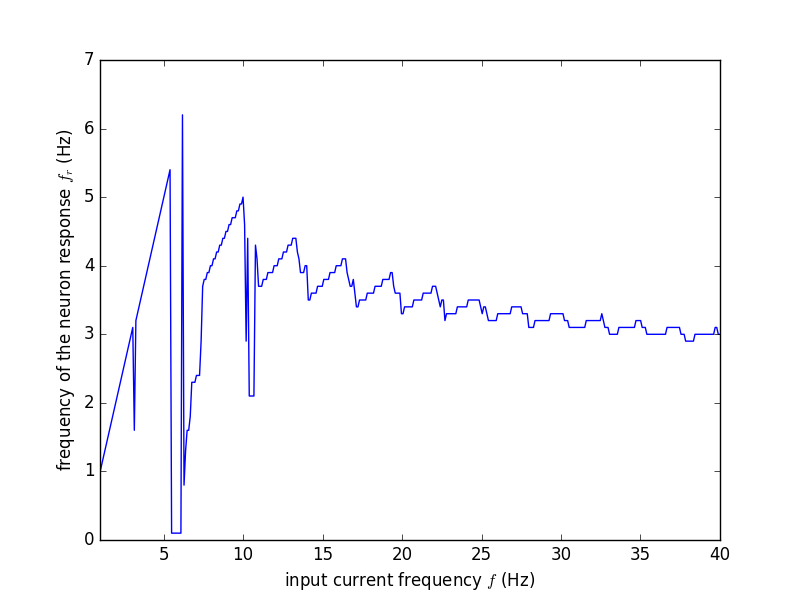
\includegraphics[width=0.7\linewidth]{LIFSin8}
  \caption{$f_r$ as a function of $f$ for a LIF neuron}
  \label{fig: LIF_f_fr}
\end{figure}

Due to technical issues, I can't guarantee that we can always find the 
real $f_r$ by using this algorithm. Therefore, the plot above is not perfect,
but it shouldn't be very far from the real curve. We see that like the firing
rate, $f_r$ doesn't code perfectly the stimulus frequency either, yet it's
still quite informative, in particular when $f$ is small. 

\subsection{conclusion}

We have spent quite some time studying the leaky integrate-and-fire model
of the neuron. By using this model, we wanted to simulate the generation
of individual spike. We supposed that the neuron is somehow accumulating
the input current and when a threshold is reached, it fires a spike.
We added also refractory period and neuronal noise in our model and spike
trains that are similar to those in real data 
(\autoref{fig: real_spike_trains} versus \autoref{fig: sim_spike_trains}) 
were generated. The model was tested with constant and sinusoidal
input current and we saw that it's quite a difficult question to understand
how information of the input stimulus is encoded by the neuron.

\iffalse

\fi
